\synctex=1
\documentclass[a4paper,11pt]{article}
\usepackage[a4paper,margin=2.7cm]{geometry}
\usepackage[utf8]{inputenc}
\usepackage{graphicx}
\usepackage{natbib}
\usepackage{authblk} % author affiliations
\usepackage[iso,english]{isodate}
\usepackage{nameref}
\newcommand*{\qref}[1]{\hyperref[{#1}]{\textit{``\nameref*{#1}'' (section \ref*{#1})}}}
\newcommand*{\qrefP}[1]{\hyperref[{#1}]{\textit{``\nameref*{#1}'', section \ref*{#1}}}}
\newcommand*{\qrefS}[1]{\hyperref[{#1}]{section \textit{\ref*{#1},
      ``\nameref*{#1}''}}}
\usepackage{lscape}
\usepackage{longtable}
\usepackage[dvipsnames,table]{xcolor}
\usepackage{latexgit}

\usepackage{hyperref}

\hypersetup{
  colorlinks = true,
  citecolor=  black,
  linkcolor = {blue},
  filecolor = cyan %% controls color of external ref, if used
}
\title{EvAM-Tools: additional documentation}

\date{\today \\ Version \gitcommithash}


\author[1,2,$\dagger$]{Ramon Diaz-Uriarte}
\affil[1]{Dpt. of Biochemistry, School of Medicine, Universidad Autónoma de Madrid, Madrid, Spain}
\affil[2]{Instituto de Investigaciones Biomédicas `Alberto Sols'
  (UAM-CSIC), Madrid, Spain}
\affil[$\dagger$]{To whom correspondence should be addressed: \normalfont r.diaz@uam.es}


\begin{document}



\begin{titlepage}
\maketitle
\tableofcontents
\end{titlepage}


\section{Introduction}

This document provides additional documentation about EvAM-Tools; some of the sections complement the Shiny web GUI application help, others apply to the package, or to both. You can run the web app from \url{https://iib.uam.es/evamtools/} or download a Docker image from \url{https://hub.docker.com/r/rdiaz02/evamshiny}; to run the R package download a Docker image from \url{https://hub.docker.com/r/rdiaz02/evamrstudio}.


\section{Cancer Progression Models included in EvAM-Tool: details}

\subsection{Cancer Progression Models and cross-sectional data: overview}

(Note: this subsection repeats material available from the landing page of the web app: \url{https://www.iib.uam.es/evamtools/#helpcsd} )

In cross-sectional data a single sample is obtained from each subject or patient. That single sample represents the "observed genotype" of, for example, the tumor of that patient. Genotype can refer to single point mutations, insertions, deletions, or any other genetic modification. As is often done by CPM software, we think of the cross-sectional data as being stored in a matrix, where rows are patients or subjects, and columns are genes; the data is a 1 if the event (or alteration or mutation) was observed and 0 if it was not.  

Note that we have talked about  "genotype" and "mutation", but CPMs have been used with non-genetic data too, and thus our preference for the expression "event accumulation models"; the key idea is that events or alterations are gained one by one, but not lost, and that we can consider the different subjects/patients in the cross-sectional data as replicate evolutionary experiments or runs where all individuals are under the same constraints (e.g., genetic constraints if we are dealing with mutations).


Cancer progression models (CPMs) or, more generally, event accumulation models, use these cross-sectional data to try to infer restrictions in the order of accumulation of events; for example, that a mutation on gene B is always preceded by a mutation in gene A (maybe because mutating B when A is not mutated). Inferring restrictions, in the sense just explained (B only if A), is what CBN, OT, OncoBN, and H-ESBCN do. 

Other cancer progression models, such as MHN, instead of modeling deterministic restrictions, model facilitating/inhibiting interactions between genes, for example that having a mutation in gene A makes it very likely to gain a mutation in gene B. 



\subsection{Cancer Progression Models (CPMs): assumptions}

CPMs assume that the observations in the cross-sectional data set are independent realizations of evolutionary processes where the same constraints hold for all tumors; therefore, a cross-sectional data set is considered a set of replicate evolutionary experiments where all individuals are under the same (genetic) constraints \citep{gerstung2011temporal, Beerenwinkel2014, beerenwinkel_computational_2016, diaz2019every}. The objective of CPMs is to infer these constraints. CPMs assume that events are gained one by one (no simultaneous acquisition of events)  and that there is no back mutation so that once gained an event is not lost; CPMs also assume that the events that drive the process (driver genes if we are thinking about cancer) are known and present in the data set. Finally, CPMs assume that all subjects start the evolutionary process without any of the studied events (i.e., all subjects start the process with 0s in the matrix of subjects by alterations). If we think about cancer, this means that ``CPMs assume that all tumors start cancer progression without any of the mutations considered in the study (the above matrix of subjects by driver alterations), but other mutations could be present that have caused the initial tumor growth'' \citep{diaz2019every}; these other additional mutations that lead to the initiation of the process are absorbed in the root node from which cancer starts \citep{Attolini2010a}.



\subsection{Cancer Progression Models (CPMs): details}


\begin{description}
\item[Oncogenetic Trees (OT)]  With OTs, restrictions in the accumulation of mutations (or events) are represented as a tree. Hence, a parent node can have many children, but children have a single parent: therefore, an event can only directly depend on another event. OTs are untimed: edge weights represent conditional probabilities of observing a given mutation, when the sample is taken, given the parents are observed. 



As detailed in \cite[p.~5 of][]{Szabo2008}, the estimation of the topology uses an ``(...) algorithm [that] takes a greedy bottom-up approach: it assigns the parent of
each node by finding the maximum-weight in-edge starting from the leaves.'' and that provides a computationally fast way of inferring the tree. 

OTs were originally in \cite{desper1999inferring}; additional references include \cite{Szabo2008, OTpackage}. Sufficient conditions for the reconstruction of the true tree when there are false positive and false negative errors are given in \cite{Szabo2002}.

which, in the absence of false observations, is guaranteed to reconstruct the original tree (if the data do conform to a tree).

Estimation of parameters ...



\end{description}




\section{Predicted genotype frequencies}
\label{pred-gen-freq}

\subsection{Predicted genotype frequencies for CBN, MCCBN, MHN, H-ESBCN}
\label{predicted-cbn-et-al}

For CBN, MCCBN, MHN, and H-ESBCN, the transition rate matrix describes the true process that generates genotypes and this matrix can be obtained from the parameters of the model ($\theta$s for MHN, $\lambda$s for the rest). Therefore, we can use the transition rate matrix to calculate the predicted probabilities of the different genotypes using standard results from continuous-time Markov Chains. In all cases here, we assume that the time of observation is exponentially distributed with rate 1 (as in \citealp{gerstung2009quantifying} or \citealp{schill2020modelling})\footnote{There is code in \texttt{evamtools}, in function \texttt{population\_sample\_from\_trm}, to obtain samples at arbitrary collections of times ---i.e., not limited to  times exponentially distributed  with rate 1.}.


Obtaining the transition rate matrix from the model output is detailed in \cite{montazeri2016large} for CBN and \cite{schill2020modelling} for MHN; for H-ESBCN see \qrefS{hesbcn}.


Once we have obtained the transition rate matrix, the fastest way to obtain the predicted genotype probabilities is using equation 4 in
\cite{schill2020modelling}; this is implemented in the non-exported function \texttt{probs\_from\_trm}, and follows also what is done in the original \texttt{Generate.pTh} from \cite{schill2020modelling}. \texttt{probs\_from\_trm} is called from function \texttt{evam}.


Instead of using that expression, we can sample from the continuous-time Markov Chain using standard procedures (\citealp[e.g., ch.~5 in][]{wilkinson2019stochastic} or \citealp[Algorithm 1 in][]{gotovos2021}). Sampling is what we do when you call \texttt{sample\_CPMs} asking for \texttt{obs\_genotype\_transitions} or \texttt{state\_counts} to be returned (and this sampling is implemented in the non-exported function \texttt{population\_sample\_from\_trm}, and called, as needed, by \texttt{sample\_CPMs}).




\subsection{Predicted genotype frequencies for OT and OncoBN}
\label{predicted-ot-oncobn}

OT and OncoBN do not return rates of a continuous-time Markov chain, but probabilities of seeing specific alterations at the time of observation. 
Predicted probabilities of genotypes for OT and OncoBN are obtained using the weights (OT) or $\theta$s (OncoBN), according to the expression for the probability of observing a genotype. For example, see section 2.2 in \cite{Szabo2008} for OT and Figure 1 and section 2.1 in \cite{nicol2021oncogenetic} for OncoBN. For OT we can use function \texttt{distributiion.oncotree} in package \texttt{Oncotree} and for OncoBN function \texttt{Lik.genotype} from package \texttt{OncoBN}\footnote{Though for OncoBN we do not use \texttt{Lik.genotype} directly, as that would involve making the exact same repeated set of calls for every individual; see the non-exported function \texttt{DBN\_prob\_genotypes} in file \texttt{onco-bn-process.R}}.

In OT observation error is already part of the model  (in contrast to what happened in CBN, MHN, H-ESBCN). This is explained in \qrefS{error_models}.

\vspace*{15pt}

For all methods, once we have the predicted probabilities, we can obtain a finite sample and, if we want, add observational (or genotyping) noise; see \qrefS{error_models}.


\section{Probabilities of evolutionary paths and transition probabilities}\label{probpaths}

How to obtain probabilities of evolutionary paths is detailed in \cite{hosseini2019a} and \cite{diaz2019every} (see S4\_Text: \url{https://doi.org/10.1371/journal.pcbi.1007246.s006}, section 3). For transition probabilities see also \cite{diaz2021conditional} (specifically section 1 in S1 Appendix: \url{https://doi.org/10.1371/journal.pcbi.1009055.s001}).


\section{Generating random CPM/EvAM models, sampling from them, and error models}\label{sec:random_evam}


\subsection{Generating random CPM/EvAM models and sampling from them}\label{subsec:random_evam}
We often want to generate data under the model of a CPM. Common use cases are:

\begin{itemize}
\item Understand what different models imply about how the cross-sectional data looks like.

\item Examine how well a method can recover the true structure when the data fulfills the assumptions of a method. For instance, we would generate data under a particular model and see if the method that implements that model can recover the true structure under different sample sizes.

\item Examine how a given method works, and what type of inferences it performs, when data are generated under the model of another method. For example, what is the output from MHN if the data are really coming from an H-ESBCN model?
\end{itemize}


Addressing the above needs involves:


\begin{enumerate}
\item Generating a random model.
 
\item Obtaining the predicted genotype frequencies from that model (see \qrefP{pred-gen-freq}).
 
\item Obtaining a finite sample from the predicted frequencies of that model.
  
\item Using the data to answer whichever questions we had; for example, analyze the sampled data with another or the same method, plot the genotype frequencies, etc.
  
\end{enumerate}



We explain each one in turn below, with reference to \texttt{evamtools} functions and arguments.

\begin{enumerate}
\item Generating a random model.
  
  Function \texttt{generate\_random\_evam} generates random models for OT, OncoBN, CBN, MHN, OncoBN, and H-ESBCN. Details about the arguments of the function are provided in its help page. No specific provision is made for randomly generating from MCCBN, as the way to simulate is similar to CBN (generate a random poset and a random set of lambdas).

\item Obtaining the predicted genotype frequencies from that model.
  
  These are returned as part of the output of \texttt{generate\_random\_evam} (as well as part of the output of \texttt{evam}). In all cases, the predicted distribution of genotypes for a model is done assuming perfect compliance with the model; we explain the general process in \qref{pred-gen-freq} and see also further details below.

\item Obtaining a finite sample from the predicted frequencies of that model.

  As the output from \texttt{generate\_random\_evam} is the same (except for the data components) to that from \texttt{evam} we can pass the model to function \texttt{sample\_CPMs}.

  When obtaining a finite sample, we can add sampling noise to the data. For example, noise due to genotyping errors; the probability of errors is controlled by argument \texttt{obs\_noise} in the call to \texttt{sample\_CPMs}.

  In more detail, the process involves:
  \begin{enumerate}
  \item Obtaining a finite sample without errors from the predicted genotype frequencies.
  \item If requested (i.e., if \texttt{obs\_noise > 0}), flipping a fraction \texttt{obs\_noise} of the observations (i.e., turning 1s to 0s and 0s to 1s).
  \end{enumerate}
  
\item Using the data to answer whichever questions we had; for example, analyze the sampled data with another or the same method, plot the genotype frequencies, etc.

  To make this simpler, function \texttt{sample\_CPMs} can return the finite sample (with or without observation noise) as a typical cross-sectional data set: a matrix where each row is a "sampled genotype", in which 0 denotes no alteration and 1 alteration in the gene of the corresponding column. This data matrix can be used directly as input for CPM methods, for instance as argument \texttt{x} (the cross-sectional data) to function \texttt{evam}.

  
\end{enumerate}

  
\subsection{Error models}
\label{error_models}

We explained above that when obtaining the predicted frequencies under a model we assume perfect compliance with the model. This is straightforward with most methods, but not with others. This summarizes the error models for each method:

\begin{description}
\item[CBN] In H-CBN the $\lambda$s describe the true underlying model that produces the true, hidden genotypes, but the observed genotypes might differ from the true ones because of observation error, for instance genotyping error  \cite[p.~2810]{gerstung2009quantifying}.
\item[H-ESBCN] As for CBN \cite[p.~756]{angaroni2021}.
\item[MHN] As for CBN (e.g., description of the simulation process in p.~244 of \citealp{schill2020modelling}).
\item[MC-CBN] With MC-CBN the model is a mixture between the CBN model and a noise component model \cite[p.~i730-i731]{montazeri2016large}. The simulations in \url{https://github.com/cbg-ethz/MC-CBN}, however, use a procedure where observations are generated from an underlying poset with a given set of lambdas, and symmetric error is then added (see the functions \texttt{mccbn:::random\_poset} and \texttt{mccbn:::random\_posets}).
\item[OncoBN] The model includes a DBN (disjunctive) or CBN (conjunctive) model, as given by a DAG and a set of $\theta$s, and a ``spontaneous activation model'' \cite[p.~3-4]{nicol2021oncogenetic}. The ``spontaneous activation model'', with parameter $\epsilon$, represents deviations from the model and allows child mutations to appear even if the parents in the DAG have not been mutated (i.e., even if the restrictions encoded in the DAG are not satisfied).
  
\item[OT] There are two sources of deviations from the OT model: a) those that result from observational (or genotyping) errors, that can lead to both false positive and false negative observational errors; b) events occurring that do not respect the OT model \cite{Szabo2002}. The second would be the same as the ``spontaneous activation'' in OncoBN.
  
  The \texttt{oncotree.fit} function in the \texttt{Oncotree} package returns a \texttt{eps} component with the estimated false positive, \texttt{epos}, and false negative, \texttt{eneg}, error rates. But these are the result of combining the two sources of error \cite{Szabo2008}: observation errors and true deviations from the model. So observation error is reflected in both \texttt{eneg} and \texttt{epos}, whereas true deviations from the model are only reflected in \texttt{epos}. In other words, the false negatives, as measured by the estimated  \texttt{eneg}, are due purely to observation error. But the \texttt{epos} are not equivalent to the $\epsilon$ of OncoBN: \texttt{epos} includes both observation error (false positives) and true mutations that occur without respecting the restrictions of the OT DAG (tree). 
  
\end{description}


\subsection{Error models and simulating and sampling from OT}
\label{error_ot}
Given the above, when sampling from a model, in all cases except OT, we have always followed the same procedure:  we have first generated observations under the true model and, if requested, then added noise. For OT, since \texttt{epos} reflects both observation and true deviations from the model, this is not possible. Thus, for OT there is a difference when we sample from a random model and when we sample from the predictions of a fitted model.

The fitted model for OT, when fitting a true data set, includes both \texttt{epos} and \texttt{eneg}. Predictions are obtained using function \texttt{Oncotree::distribution.oncotree} with, by default, argument \texttt{with.errors = TRUE}, which is what argument \texttt{with\_errors\_dist\_ot = TRUE} to \texttt{evam} does. Therefore, from a fitted model, the predictions incorporate both false positive and false negative error rates, as estimated by \texttt{oncotree.fit}; as explained above, however, these estimated error rates are both the errors from the observational process (genotyping errors, for example) and true deviations from the model. When you later call \texttt{sample\_CPMs} you can add an \texttt{obs\_noise} with value larger than 0, but for OT, when sampling from the model fitted to observed data this might not make sense (since \texttt{epos} and \texttt{eneg} have been used already to produce the predicted genotype frequencies). Thus, if we use \texttt{with\_errors\_dist\_ot = TRUE} in the \texttt{evam} call and then set \texttt{obs\_noise = 0} when calling \texttt{sample\_CPMs}, the observed data we generate should be the same (have the same distribution) as if we had used \texttt{Oncotree::generate.data} with \texttt{method = ``D1''}, \texttt{with.errors = TRUE} and \texttt{edge.weights = ``estimated''}.\footnote{
  We can try to divide the \texttt{epos} component in a component like OncoBN's $\epsilon$ and another noise component. Then, we would first obtain the predicted distribution via \texttt{distribution.oncotree} with the $\epsilon$-like (and with \texttt{eneg} = 0), sample, and add noise. If \texttt{epos} $>$ \texttt{eneg} we can do this so that the noise added is symmetrical. This is shown in function \texttt{dot\_noise\_gd\_3} in \texttt{inst/miscell/OT\_generate\_data\_sample\_CPMs.R}.

  
In that same file \texttt{inst/miscell/OT\_generate\_data\_sample\_CPMs.R} we show that a model obtained from \texttt{generate\_random\_evam} with \texttt{ot\_oncobn\_eps}  $= x$ and sampled using \texttt{sample\_CPMs} with \texttt{obs\_noise} $= y$ gives predictions with the same distribution as if we had used \texttt{Oncotree::generate.data} on that very same oncotree object but with \texttt{epos} = $x + y - (1/2)\ x\ y$ and \texttt{eneg} = $y$.}



When sampling from a random model, using \texttt{generate\_random\_evam}, we generate the tree (the DAG) with density as given by argument \texttt{graph\_density} and the weights from uniform distributions with limits  given by \texttt{ot\_oncobn\_weight\_min} and \texttt{ot\_oncobn\_weight\_max}. In addition, we can set a value larger than 0 for \texttt{ot\_oncobn\_epos}. This will be used as the \texttt{epos}, but not \texttt{eneg}, value of the OT model. When you sample and optionally add noise, with argument \texttt{obs\_noise} to function \texttt{sample\_CPMs} noise is added symmetrically. Thus, we use a procedure where \texttt{ot\_oncobn\_epos} behaves as OncoBN's $\epsilon$ and \texttt{obs\_noise} is purely symmetric observational error.


Why this difference? When you use a model fitted to real data, it is sensible to use \texttt{Oncotree}'s inferential machinery to estimate the \texttt{epos} and \texttt{eneg}. If you later want to generate samples, these already include deviations from the model and noise. However, when you simulate a model, there is no data and thus no way to estimate  \texttt{epos} and \texttt{eneg}. Therefore, it is sensible to split errors into two distinct pieces, which is also coherent with what we do with the rest of the methods: deviations from the model, and noise.



%% I only understand the meaning of a few combinations:
%% D1 and D2, these are the equivalent calls.
% d1 <- generate.data(3e5, ov.tree, with.errors = TRUE, method = "D1",
%                     edge.weights = "estimated")
% d3 <- generate.data(3e5, ov.tree, with.errors = TRUE, method = "D2",
% edge.weights = "estimated")


%% So with errors, D2, estiamted, which calls dist.oncto w/o errors, but using estimated, and then adds the errors.

%% The thing is that distribution.oncotree uses, correctly, the errors. 




\section{Random EvAM models and transitive reduction}
\label{sec:random-evam-models}

As of now, the generation of random EvAM models uses transitively reduced graphs (we call \texttt{mccbn::random\_poset} with argument \texttt{trans\_reduced = TRUE}). This does not decrease the number of models that can be expressed when using CBN. However, it can limit the range of models when we can mix AND, OR, XOR in the same model. The following  examples illustrate how this makes certain models impossible.


\begin{figure}[h!]
%  \centering
  \hspace*{-1.8cm}
  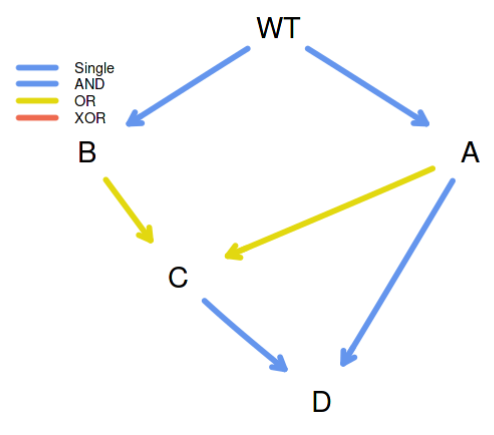
\includegraphics[width=.35\linewidth]{./dag2.png}
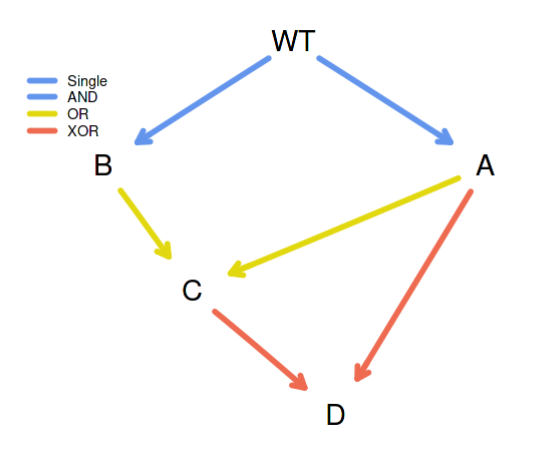
\includegraphics[width=.35\linewidth]{./dag3.png}
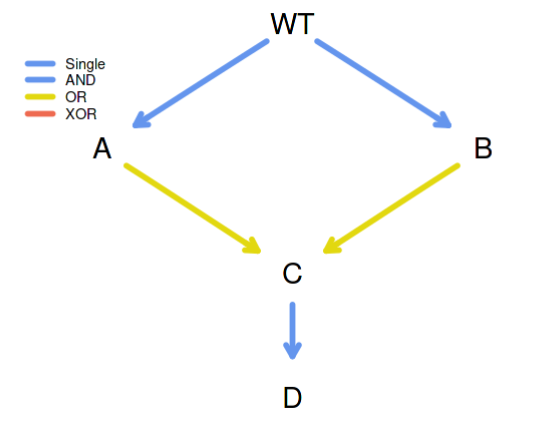
\includegraphics[width=.35\linewidth]{./dag1.png}
\caption{Non-transitively reduced DAG, OR and AND (left),
  non-transitively reduced DAG, OR and XOR (center),
  transitively reduced DAG.}\label{dag2}
\end{figure}

\begin{itemize}
\item Under the left-most DAG in Fig.~\ref{dag2} we cannot observe genotype BCD.
\item Under the center DAG in Fig.~\ref{dag2} we cannot observe genotype ACD.
\item Under the right-most DAG, which is the transitive reduction of the above two graphs, we can observe both BCD and ACD.
\end{itemize}


% \begin{figure}[h!]
% \centering
% 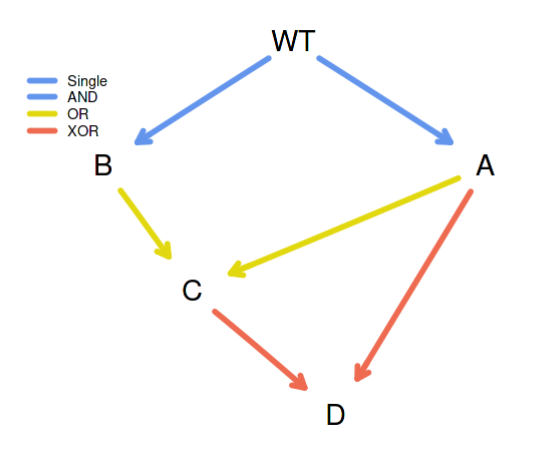
\includegraphics[width=.43\linewidth]{./dag3.png}
% \caption{Non-transitively reduced DAG, OR and XOR}\label{dag3}
% \end{figure}

% Under the DAG in Fig.~\ref{dag3} we cannot observe genotype ACD.


% \begin{figure}[h!]
% \centering
% 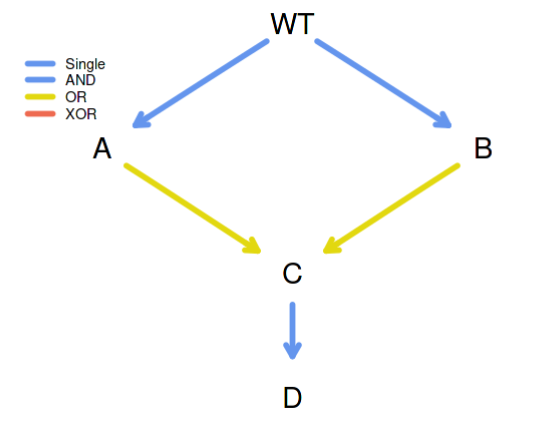
\includegraphics[width=.43\linewidth]{./dag1.png}
% \caption{Transitively reduced DAG}\label{dag1}
% \end{figure}

% Under the DAG in Fig.~\ref{dag1}, which is the transitive reduction of the above two graphs, we can observe both BCD and ACD.

Can we imagine biological scenarios where the left-most or center scenarios in Fig.~\ref{dag2} would apply? Yes. We don't recall seeing them in the literature, though. If this is deemed relevant, it is just a matter of changing  \texttt{trans\_reduced = TRUE} when we are simulating HESBCN models inside function \texttt{random\_evam}.

You can of course construct the non-transitively reduced graphs ``by hand'' (creating the data frame with the appropriate structure) or, much simpler, using the Shiny web app.



\section{H-ESBCN: details and examples of using $\lambda$s and computing transition rate matrices and predicted genotype frequencies}\label{hesbcn}

Here I provide full details about how we interpret and use the results from the method described in \cite{angaroni2021}. I do this here because, in contrast to CBN or MHN, there is no existing previous code or examples that do this, and we found some potentially confusing issues. I have made a specific section so as not to break the flow of the former sections.


\subsection{Lambdas from the output: "Best Lambdas" and "lambdas\_matrix"}

The output returned by the H-ESBCN C code contains a "Best Lambdas" vector. The output returned by function \texttt{import.hesbcn} (that we have included in the code, in file \texttt{HESBCN\_\_import.hesbcn.R}) has an object called "lambdas\_matrix" where each of the lambdas for a gene is divided by the number of parents. This can be checked in any of the examples in the PMCE repository. Code that shows three examples, with XOR, OR, AND is available under "inst/miscell/examples/HESBCN-lambdas-from-examples.R".


It is the output from "Best lambdas" (i.e., the undivided lambdas) that are "[the] rates of the Poisson processes of the continuous-time HMM, associated with the vertices of the model, which allow one to estimate the expected waiting time of a node, given that its predecessor has occurred." (p. 756). (What is the division? An  operation that modifies an internal data structure, and just a temporary operation, done merely for implementation purposes. In line 95 of the code ---as of current version, in \url{https://github.com/BIMIB-DISCo/PMCE/blob/main/Utilities/R/utils.R}--- the divided lambdas are again summed, so the partition disappears: "curr\_in\_lambda = sum(hesbcn\$lambdas\_matrix[,curr\_node])", and it is that value that is used in further downstream computations;  email with the authors on 2021-07-09). The ``Best lambdas'' are returned by our modified \texttt{import.hesbcn} function.


\subsection{Interpreting OR and XOR (and AND)}

I find Figure 1C  of  \cite{angaroni2021} possibly confusing. First, the non-confusing part:  node "D" has a rate when exactly one of B XOR C has occured, and node "G" some other rate when E or F or both E and F have occurred. (Note: the figure shows $\tau$s, not $\lambda$s. The comments here refer to the $\lambda$s).


Now the (for me, at least) possibly confusing part: it seems that the node called "B xor C" is such that B and C have the same rates of dependencies on A; in other words, it would seem to imply that \(\lambda_B = \lambda_C\). Similarly, the node called "E or F" seems to indicate that both E and F have the same rate, so \(\lambda_E = \lambda_F\). But this need not be so. In fact, virtually all of the examples we have looked at, and the examples in their output, do not satisfy that the rates to the genes that are part of a XOR, OR, or AND relationship are the same. For instance, in the example above of Bladder Urothelial Carcinoma (see "inst/miscell/examples/HESBCN-lambdas-from-examples.R"), KMT2D depends on KMT2C and TP53, but the rate for KMT2C, \(\lambda_{KMT2C} = 0.1991\) and that for TP53, \(\lambda_{TP53} = 0.8062\).


Remember that the \(\lambda\) for a gene is the rate of the process until that mutation appears and is fixated, given all the dependencies of that gene are satisfied (which is, of course, the same interpretation as under CBN). Again:  "[the] rates of the Poisson processes of the continuous-time HMM, associated with the vertices of the model, which allow one to estimate the expected waiting time of a node, given that its predecessor has occurred." (p. 756).

But the rate at which the parents are satisfied can differ (as it was the case for CBN). A difference with respect to CBN is that, with CBN, if a gene D depends on three genes A, B, C, regardless of the lambdas of each of A, B, C, D can only happen once all of A, B, C are present. With H-ESBCN and with OR and XOR relationships this is no longer the case: one can see D with only A, for example.


What if some genes depend with and AND, others with a XOR and other with a OR? Just apply the rules to each type of dependency: in the HESBCN model if a gene depends on a set of genes, it has the same type of dependency on all the genes of that set.

\subsection{Predicted genotype frequencies}
\label{sec:pred-genotype-freq}

Once we have the transition rate matrix, obtaining the predicted genotype frequencies uses the same procedure as for CBN and MHN; see \qrefS{predicted-cbn-et-al}.



\subsection{An example with OR and XOR}
\label{sec:org6769f8f}
In this example:

\begin{itemize}
 \item A, B, C depend on none.
 \item D depends, with an OR, on both A and B
 \item E depends, with an XOR, on B and C
 \item Transition rate matrix is shown below: rows are origin, column destination. $\lambda$s are those from "Best Lambdas".
 \end{itemize}

 \begin{landscape}
 \begin{table}[ht]
   \rowcolors{2}{gray!25}{white}
\centering
\begin{tabular}{rlllllllllllllllllllll}
  \hline
 & WT & A & B & C & AB & AC & AD & BC & BD & BE & CE & ABC & ABD & ABE & ACD & ACE & BCD & BDE & ABCD & ABDE & ACDE \\ 
  \hline
WT &  & $\lambda_A$ & $\lambda_B$ & $\lambda_C$ &  &  &  &  &  &  &  &  &  &  &  &  &  &  &  &  &  \\ 
  A &  &  &  &  & $\lambda_B$ & $\lambda_C$ & $\lambda_D$ &  &  &  &  &  &  &  &  &  &  &  &  &  &  \\ 
  B &  &  &  &  & $\lambda_A$ &  &  & $\lambda_C$ & $\lambda_D$ & $\lambda_E$ &  &  &  &  &  &  &  &  &  &  &  \\ 
  C &  &  &  &  &  & $\lambda_A$ &  & $\lambda_B$ &  &  & $\lambda_E$ &  &  &  &  &  &  &  &  &  &  \\ 
  AB &  &  &  &  &  &  &  &  &  &  &  & $\lambda_C$ & $\lambda_D$ & $\lambda_E$ &  &  &  &  &  &  &  \\ 
  AC &  &  &  &  &  &  &  &  &  &  &  & $\lambda_B$ &  &  & $\lambda_D$ & $\lambda_E$ &  &  &  &  &  \\ 
  AD &  &  &  &  &  &  &  &  &  &  &  &  & $\lambda_B$ &  & $\lambda_C$ &  &  &  &  &  &  \\ 
  BC &  &  &  &  &  &  &  &  &  &  &  & $\lambda_A$ &  &  &  &  & $\lambda_D$ &  &  &  &  \\ 
  BD &  &  &  &  &  &  &  &  &  &  &  &  & $\lambda_A$ &  &  &  & $\lambda_C$ & $\lambda_E$ &  &  &  \\ 
  BE &  &  &  &  &  &  &  &  &  &  &  &  &  & $\lambda_A$ &  &  &  & $\lambda_D$ &  &  &  \\ 
  CE &  &  &  &  &  &  &  &  &  &  &  &  &  &  &  & $\lambda_A$ &  &  &  &  &  \\ 
  ABC &  &  &  &  &  &  &  &  &  &  &  &  &  &  &  &  &  &  & $\lambda_D$ &  &  \\ 
  ABD &  &  &  &  &  &  &  &  &  &  &  &  &  &  &  &  &  &  & $\lambda_C$ &  &  \\ 
  ABE &  &  &  &  &  &  &  &  &  &  &  &  &  &  &  &  &  &  &  & $\lambda_D$ &  \\ 
  ACD &  &  &  &  &  &  &  &  &  &  &  &  &  &  &  &  &  &  & $\lambda_B$ &  & $\lambda_E$ \\ 
  ACE &  &  &  &  &  &  &  &  &  &  &  &  &  &  &  &  &  &  &  &  & $\lambda_E$ \\ 
  BCD &  &  &  &  &  &  &  &  &  &  &  &  &  &  &  &  &  &  & $\lambda_A$ &  &  \\ 
  BDE &  &  &  &  &  &  &  &  &  &  &  &  &  &  &  &  &  &  &  & $\lambda_A$ &  \\ 
  ABCD &  &  &  &  &  &  &  &  &  &  &  &  &  &  &  &  &  &  &  &  &  \\ 
  ABDE &  &  &  &  &  &  &  &  &  &  &  &  &  &  &  &  &  &  &  &  &  \\ 
  ACDE &  &  &  &  &  &  &  &  &  &  &  &  &  &  &  &  &  &  &  &  &  \\ 
   \hline
\end{tabular}
\end{table}
 \end{landscape}


\subsection{Three examples from actual analysis}
\label{sec:orgdc3f991}
\begin{itemize}
\item The code in inst/miscell/HESBCN-OR-XOR-AND-lambda-and-rates.R contains examples of how we use those lambdas (the \texttt{n}, number of steps, used is ridiculously small, and just for the sake of speed).
\end{itemize}
\begin{enumerate}
\item OR
\label{sec:org9d47997}
\begin{itemize}
\item Suppose output such as this (again, see file inst/miscell/HESBCN-OR-XOR-AND-lambda-and-rates.R for how to reproduce it).
\end{itemize}

\begin{verbatim}
 $adjacency_matrix
      Root A B C D
 Root    0 1 1 0 0
 A       0 0 0 1 1
 B       0 0 0 1 1
 C       0 0 0 0 0
 D       0 0 0 0 0

 $lambdas_matrix
      Root     A     B     C      D
 Root    0 8.083 2.585 0.000 0.0000
 A       0 0.000 0.000 8.914 0.2062
 B       0 0.000 0.000 8.914 0.2062
 C       0 0.000 0.000 0.000 0.0000
 D       0 0.000 0.000 0.000 0.0000


 $parent_set
        A        B        C        D 
 "Single" "Single"    "XOR"     "OR" 


 $lambdas
 [1]  8.0833  2.5854 17.8277  0.4124

 $edges
   From To      Edge Lambdas Relation
 1 Root  A Root -> A  8.0833   Single
 2 Root  B Root -> B  2.5854   Single
 3    A  C    A -> C 17.8277      XOR
 4    B  C    B -> C 17.8277      XOR
 5    A  D    A -> D  0.4124       OR
 6    B  D    B -> D  0.4124       OR

\end{verbatim}

\begin{itemize}
\item From the above output, these are the lambdas: $\lambda_A = 8.0833, \lambda_B = 2.5854, \lambda_C = 17.8277, \lambda_D = 0.4124$.
\item Focusing only on A, B, D, to see gene D we can follow four paths.
\begin{itemize}
\item The first two involve only two mutations:
\begin{itemize}
\item \(WT \rightarrow A \rightarrow AD\)
\item \(WT \rightarrow B \rightarrow BD\)
\item The first is much faster, since the rate for the transition from WT to A is 8.1 compared to 2.6 of the transition B to D (from competing exponentials, the probabilities of moving to A and B are 0.76 and 0.24, respectively).
\end{itemize}
\item In the other two paths D is the third gene to appear:
\begin{itemize}
\item \(WT \rightarrow A \rightarrow AB \rightarrow ABD\)
\item \(WT \rightarrow B \rightarrow AB \rightarrow ABD\)
\item These two paths take the same time, on average: both A and B need to appear (with rates given by \(\lambda_A\), \(\lambda_B\)) and then we need D to appear (\(\lambda_D\)).
\end{itemize}

\item Similarly, to get to genotype "A, B, D" we can follow these paths:
\begin{itemize}
\item \(WT \rightarrow A \rightarrow AB \rightarrow ABD\)
\item \(WT \rightarrow B \rightarrow AB \rightarrow ABD\)
\item \(WT \rightarrow A \rightarrow AD \rightarrow ABD\)
\item \(WT \rightarrow B \rightarrow BD \rightarrow ABD\)
\item All of them take the same expected time, as we need A, B, and D to happen, each governed by \(\lambda_A\), \(\lambda_B\), \(\lambda_D\), respectively.
\end{itemize}
\end{itemize}
\item In terms of fitness, if we used OncoSimulR (see additional document ``Using OncoSimulR to get accessible genotypes and transition matrices''), we would write, for the fitness of AB: \((1 + \lambda_A) (1 + \lambda_B)\), for AD \((1 + \lambda_A) (1 + \lambda_D)\), and for ABD \((1 + \lambda_A) (1 + \lambda_B) (1 + \lambda_D)\).
\begin{itemize}
\item Note, specifically, that genotypes \(AD\) and \(BD\) are not fitness equivalent, unless \(\lambda_A = \lambda_B\).
\end{itemize}
\end{itemize}
\item XOR
\label{sec:orgc1e93a8}
\begin{itemize}
\item Using the above example, and focusing only on A, B, C, these are the only ways of seeing a C:
\begin{itemize}
\item \(WT \rightarrow A \rightarrow AC\)
\item \(WT \rightarrow B \rightarrow BC\)
\item As we have a XOR, no routes can go through AB.
\item The first is much faster and common than the second (\(\lambda_A = 8.1; \lambda_B = 2.6\)).
\item Fitness (again, this is relevant if using, for example, OncoSimulR) of \(AC\) is \((1 + \lambda_A) (1 + \lambda_C)\) and of \(BC\) \((1 + \lambda_B) (1 + \lambda_C)\).
\end{itemize}
\end{itemize}

\item Both OR and XOR
\label{sec:org5edd44b}
\begin{itemize}
\item There is nothing new. As an example, gaining both C and D mutations.
\begin{itemize}
\item \(WT \rightarrow A \rightarrow AC \rightarrow ACD\)
\item \(WT \rightarrow B \rightarrow BC \rightarrow BCD\)
\item \(WT \rightarrow A \rightarrow AD \rightarrow ACD\)
\item \(WT \rightarrow B \rightarrow BD \rightarrow BCD\)
\item There is no path going through \(AB\) since C has a XOR relationship on A and B.

\item In the first path we first need to wait for A to happen (rate \(\lambda_A\)) then C (\(\lambda_C\)) then D (\(\lambda_D\)).
\item Same for the second, with B instead of A. The first path is much more common than the second.
\item The third path transposes the order of occurrence of D and C, but takes the same average time as the third. Note that the fitness of the final genotype is the same through both routes, only the order of steps changes.
\item The fourth path transposes the order of occurrence of D and C, but takes the same average time as the fourth. Note that the fitness of the final genotype is the same through both routes, only the order of steps changes.
\end{itemize}
\end{itemize}
\end{enumerate}

\subsection{Combining AND, OR, XOR?}
\label{sec:org78cffb2}
Nothing changes. Use the rules for AND where there is an AND, XOR where there is a XOR, OR where there is an OR. Again, in the HESBCN model if a gene depends on a set of genes, it has the same type of dependency on all the genes of that set.

\clearpage


\section{Shiny EvAM-Tools web app}
\subsection{Building the models and example data}
\label{sec:build-models-example}

\subsubsection{Example data/DAGs/MHNs}
\label{sec:exampe-datadagsmhns}

For each of the ways to input cross-sectional data or build models, we provide some pre-built examples. You can use these to directly run the CPMs or modify them to your liking. The MHN and DAG builders allow you start from working examples. Explanations on what is available and why follow: 

\begin{description}
\item[Modifying pre-built examples] If you modify the examples, you probably will want to give your dataset or example a distinctive name.

% If you modify a pre-built example and want to go back to the original, in your browser clean the cache and refresh.
  
\item[Cross-sectional data] We provide data sets that have been generated under specific models with AND, OR, XOR. However, no DAG is shown here, and that is on purpose; use the labels as possible hints, not as the truth, and compare with datasets you can generate from models you specify under the DAG builder.

\item[DAG] Several examples to illustrate OR/AND/XOR and mixtures of the above are provided.
  
\end{description}


\subsection{Cross-sectional data input}
\label{sec:cross-sectional-data}

\subsubsection{Number of genes and genes without mutations}
\label{sec:number-genes-genes}

 When creating user data (for instance, when adding new genotypes), any gene that has no mutations is automatically excluded from the data, regardless of the setting for number of genes. This is a feature, not a bug. For example, suppose you set the number of genes to 3, but you only specify frequencies, or counts, for genotypes "A" and "A, B". The data set will only contain columns for genes A and B (since gene C has no mutations and it would be excluded during the analyses).


 \subsection{Naming and saving data and model}
 \label{shiny-save}

 To make it easier to use and analyze different models and data sets, you can name/rename the dataset used. This is at the top of the page, under ``(Re)name the data''.

 You can save the data and models (at the bottom of the page). If you define a DAG or an MHN model, the saved object contains the model. In the case of the DAG, that includes the generated data (if any), and several components that are used by evamtools and that provide a complete description of the model. If you use MHN, what are saved are the sampled data (if any) and the log$\Theta$ matrix you entered.

\subsection{Tabular output from the Shiny app}
\label{tabular-output}

\begin{description}
\item[Transition probabilities] Conditional probability of transitions to a genotype (obtained using competing exponentials from the transition rate matrix for all methods except OT and OncoBN); for OT and OncoBN this is actually an abuse of the untimed oncogenetic tree model, as explained in \cite{diaz2019every}.
\item[Transition rates] Transition rates of the continuous-time Markov chain that models the transition from one genotype to another. This option is not available for OT and OncoBN, as these do not return rates.
\item[Predicted genotype relative frequencies] The predicted frequencies of genotypes under the model. See \qrefS{error_models} for details about OT and OncoBN
\item[Sampled genotype counts] Counts, or absolute genotype frequencies, obtained by sampling from the predicted frequencies.
  
  %% Next only if you ask for 'Sample for observed genotype transitions'
\item[Observed genotype transitions (counts)] Only if you ask for 'Sample for observed genotype transitions' in ``Advanced options and CPMs to use''. This is the number of observed transitions between genotypes.
  
\end{description}


See also further details in section \qrefS{error_models} as well as in the help for functions \texttt{evam} and \texttt{sample\_CPMs}.

\section{FAQ}
\label{sec:faq}


\subsection{Why haven't you used method X?}\label{other_methods}

We have included here what we believe are the current state-of-the-art methods that have existing public implementations that run in reasonable time. After searching the literature, we have included any method that could be deemed appropriate. We have, in fact, provided access to two very recent methods: H-ESBCN and OncoBN (and their github repos show we have contributed bug reports).

Among the remaining methods available, most of them do not seem to be developed nor used anymore. For some of these methods, their authors have developed newer methods that seem to have superseded the former methods. Some other methods  have dependencies on external libraries that are not open source.  And, of course, we cannot provide access to methods that have no software, or have software that will run only under proprietary systems. Some further comments are provided in S4\_Text in \cite{diaz2019every} (\url{https://doi.org/10.1371/journal.pcbi.1007246.s006}).

If you think we have overlooked a method that should be included, please let us know.




\subsection{With OncoBN sometimes I obtain DAGs that are not transitively reduced}

Yes, that can happen. See details here \url{https://github.com/phillipnicol/OncoBN/issues/5}.


\subsection{In the DAG figures, why do nodes with two or more incoming edges have only a single annotated edge with a number?}
\label{faq-single-num}

Because the number, which is the $\lambda$ (CBN, HESBCN) or $\theta$ (OncoBN) is the rate (CBN, HESBCN) or probability, conditional on the assumptions indicated by the DAG being satisfied. So the $\lambda$ or $\theta$ are per node, not per edge. For instance, suppose gene C depends on both A and B (there is an AND); and you see a number of 0.7. That is the $\lambda$ or $\theta$ for observing C mutated when both A and B are mutated. 


And why then not annotate the nodes, instead of the edges? Because in our experience:
\begin{itemize}
\item Annotating nodes leads to more confusing figures.
\item Annotating edges shows what transitions are likely/fast, an idea not conveyed by annotating nodes.
\end{itemize}



\subsection{Do sampled genotype frequencies and counts contain observation noise? And predicted genotype frequencies?}
\label{sec:do-sampled-genotype}

For all models except OT, predicted genotype frequencies do not have observation noise added. The OT model itself estimates noise, and thus predicted frequencies obtained from models fitted to observed data incorporate observation noise. See \qref{error_models}.

When we obtain a finite sample from the predicted frequencies, you can decide to add observation noise with argument \texttt{obs\_noise} to function \texttt{sample\_CPMs}; what happens with OT depends on whether the predictions are from a simulated model or a model fit to observed data; see details in \qref{error_ot}.




\subsection{I want to setup my own Shiny app with different default ``Advanced options''}

In file \texttt{EvAM-Tools/evamtools/inst/shiny-examples/evamtools/ui.R} search for ``Advanced options'' and modify the defaults to whatever you want.


\subsection{How can I use the Shiny app in a local intranet with load balancing using multiple Docker instances}
\label{haproxy}

This is well beyond the scope of this document and there are many options available. One that can work (and this is more or less what we actually do) is the following:

\begin{itemize}
\item Start multiple Docker instances (say, 20) by changing the range of ports, for example, 3010 to 3030.
\item Use HAProxy (\url{https://www.haproxy.org/}) so that you have a single entry point for all requests to the service that are then distributed, with load balancing, to the 20 instances. You will want to use ``sticky connections'' (see the HAProxy documentation).
\end{itemize}

As said above, this is just a sketch of the basic procedure. There are many other options.


\subsection{If I use the Docker image for the package (rdiaz02/evamrstudio), can I run the Shiny app?}

Yes, you can. Just start a browser as explained in the README (\url{https://github.com/rdiaz02/EvAM-Tools#how-to-run-the-r-package-from-the-docker-image}). Then, once in RStudio, in the R console type \verb@ runShiny() @ and you will have the interactive Shiny app open. But even if you can do it, it is not clear why you'd want to do this: if you only want to run the Shiny app, the Docker image rdiaz02/evamshiny is lighter and the steps to launch it much faster.



\subsection{Why aren't you using Shiny Server?}
\label{sec:why-arent-you}

Because we did not see it as necessary or convenient. If you want to run Shiny interactively from an R session load \texttt{evamtools} and call function \texttt{runShiny}; no need for Shiny Server.

If we want to run Shiny as a service, with Docker images it is rather straightforward to launch a bunch Docker instances and use HAProxy to access to them using load-balancing (see \ref{haproxy}) or any other such similar solution.

Moreover, notice this in the Shiny Server documentation (\url{https://shiny.rstudio.com/articles/shiny-server.html}): ``Shiny Server will host each app at its own web address and automatically start the app when a user visits the address. When the user leaves, Shiny Server will automatically stop the app. ''  That is not exactly what we want. We want the containers to be up and running, ready to answer requests as they come with minimal latency. Moreover, a single Shiny Server would have given access to a single instance of the app (so that if two or more users access the app, one of the users has to wait while R is busy executing what the other user is running); to give users access to multiple simultaneous instances we would have needed, for example, multiple Docker images each with its own Shiny Server.

However, we might be missing something; if you think Shiny Server would allow or ease some use cases, please let us know.




\subsection{I want to build my own Docker images}

If you want to modify the Docker images, modify the Dockerfiles: Dockerfile-evam-rstudio (for the RStudio Dockerfile that launches RStudio) or Dockerfile-evam-shiny (well, for the Dockerfile that creates the container to run shiny). 


Then, from the `EvAM-Tools` directory run one or both of:

\begin{verbatim}
docker build -f Dockerfile-evam-shiny  --tag somename .
docker build -f Dockerfile-evam-rstudio  --tag somename .
\end{verbatim}


You can now run these images, as explained in the README file..

Note: it is possible, and actually a better idea, to run docker without sudo; look a the Docker documentation:
\url{https://docs.docker.com/engine/security/rootless/}).


\subsubsection{What if creating the image fails because of no internet connection from the container}
Creating the above image requires installing R packages and that might fail because the Docker container cannot connect with the internet. The following might help: \url{https://superuser.com/a/1582710}, \url{https://superuser.com/a/1619378}. In many cases, doing
\verb@ sudo systemctl restart docker@ might be enough.


\subsubsection{Cleaning the build cache and stale old images}
Sometimes (e.g., if the base containers change or you want to remove build cache) you might want to issue

\begin{verbatim}
docker builder prune
\end{verbatim}

or the much more drastic

\begin{verbatim}
docker system prune -a

\end{verbatim}
Please, read the documentation for both.


\subsubsection{Copying docker images from one machine to another}
Yes, that can be done. See here, for example: \url{https://stackoverflow.com/a/23938978}


\section{License and copyright}
This work is Copyright, \copyright, 2022, Ramon Diaz-Uriarte.

Like the rest of this package (EvAM-Tools), this work is licensed under the GNU Affero General Public License. You can redistribute it and/or modify it under the terms of the GNU Affero General Public License as published by the Free Software Foundation, either version 3 of the License, or (at your option) any later version.

This program is distributed in the hope that it will be useful, but WITHOUT ANY WARRANTY; without even the implied warranty of MERCHANTABILITY or FITNESS FOR A PARTICULAR PURPOSE. See the GNU Affero General Public License for more details.

You should have received a copy of the GNU Affero General Public License along with this program. If not, see \url{https://www.gnu.org/licenses/}. 

The source of this document and the EvAM-Tools package is at \url{https://github.com/rdiaz02/EvAM-Tools}.

\bibliographystyle{natbib}
\bibliography{cpm_refs}



\end{document}
